\documentclass{article}
\usepackage[utf8]{inputenc}
\usepackage[T1]{fontenc}
\usepackage[italian]{babel}
\usepackage{geometry}
\usepackage{graphicx}
\usepackage{amsmath}
\usepackage{tabularx}
\usepackage{booktabs}
\geometry{a4paper, margin=1in}

\title{Capitolo 5 -Autenticazione Utenti}
\author{}
\date{}

\begin{document}

\maketitle

\section*{Fondamenti: Identificazione vs Autenticazione}

La base della sicurezza informatica risiede nel \textbf{controllo degli accessi}. Questo concetto implica che un soggetto sia autorizzato a compiere una determinata azione su una risorsa. Per far sì che ciò funzioni, dobbiamo essere certi dell'identità di quel "qualcuno". Il processo di determinazione dell'identità si suddivide in due fasi distinte:

\begin{itemize}
    \item \textbf{Identificazione:} l'atto di asserire chi sia un soggetto. L'utente si identifica presso il sistema presentando una credenziale, come l'ID utente.
    \item \textbf{Autenticazione:} l'atto di provare che l'identità dichiarata sia corretta, ovvero che il soggetto sia effettivamente chi afferma di essere. Il sistema verifica l'utente attraverso lo scambio di informazioni di autenticazione.
\end{itemize}

Mentre le identità sono spesso note, prevedibili o facilmente intuibili, le informazioni di autenticazione dovrebbero rimanere private. Se il processo di autenticazione non è sufficientemente robusto, l'intero sistema non può essere considerato sicuro. I meccanismi si basano su tre pilastri: qualcosa che l'utente \textbf{sa} (conoscenza), qualcosa che l'utente \textbf{è} (biometria/caratteristiche) o qualcosa che l'utente \textbf{ha} (token/possesso).

\vspace{0.8cm}

\section*{Autenticazione basata sulla Conoscenza: Le Password}

L'autenticazione basata su frasi e fatti è il meccanismo più diffuso, ma presenta notevoli difficoltà d'uso e gestione:

\begin{itemize}
    \item \textbf{Incombenza:} fornire una password per ogni accesso a un oggetto può risultare scomodo e dispendioso in termini di tempo.
    \item \textbf{Divulgazione:} se la password viene rivelata a un individuo non autorizzato, l'oggetto protetto diventa immediatamente accessibile. Per \textit{ri-proteggerlo}, l'utente deve cambiare la password e informare tutti gli altri utenti legittimi.
    \item \textbf{Revoca:} revocare il diritto di accesso a un singolo utente richiede il cambio della password per tutti, causando gli stessi disagi della divulgazione.
    \item \textbf{Perdita:} può essere impossibile recuperare una password dimenticata, a meno che l'amministratore di sistema non ne fornisca una nuova.
\end{itemize}

\vspace{0.8cm}

\section*{Gli Step di Attacco alle Password}

Un attaccante può seguire una progressione di 12 step per tentare di indovinare una password:

\begin{enumerate}
    \item Nessuna password.
    \item Password uguale allo User ID.
    \item Derivata dal nome o dall'ID dell'utente.
    \item Parole comuni (es. "password", "secret") o pattern di tastiera (es. "qwerty", "aaaaaa").
    \item Termini contenuti in un dizionario tascabile.
    \item Termini di un dizionario inglese completo.
    \item Termini di dizionari in altre lingue.
    \item Termini di dizionari con variazioni di maiuscole o sostituzioni di caratteri (es. '0' per 'O', '1' per 'l').
    \item Brute force su tutte le combinazioni alfabetiche.
    \item Brute force sull'intero set di caratteri.
\end{enumerate}

Sebbene questi step richiedano tempo, per un attaccante il tempo non è un fattore limitante. La forza di una password non risiede nella sua segretezza assoluta, ma nel numero di tentativi richiesti per indovinarla.

\vspace{0.8cm}

\section*{Debolezza del Fattore Umano}

Le password sono un mezzo economico ed efficiente, ma il loro punto debole è l'essere umano che le sceglie. Gli utenti tendono a usare pattern prevedibili o mostrano negligenza.

\vspace{0.3cm}
Le abitudini umane nella scelta delle password non siano cambiate dal 1979 a oggi.

\vspace{0.5cm}
\noindent \begin{minipage}{0.48\textwidth}
    \begin{itemize}
        \item \textbf{Dati storici (1979):} Uno studio di Morris e Thompson mostrava già una forte prevalenza di password brevi (3-6 caratteri) o basate su parole del dizionario.
        \item \textbf{Dati recenti (2019 - Dataset di 500M di password):}
        \begin{itemize}
            \item Circa il \textbf{30\%} degli utenti sceglie password con meno di sette caratteri.
            \item Quasi il \textbf{50\%} utilizza nomi, parole gergali, termini del dizionario o pattern banali (cifre consecutive, tasti adiacenti sulla tastiera).
            \item Tra le password più popolari figurano ancora "123456", "password" e "iloveyou".
        \end{itemize}
    \end{itemize}
\end{minipage}
\hfill
\begin{minipage}{0.48\textwidth}
    \centering
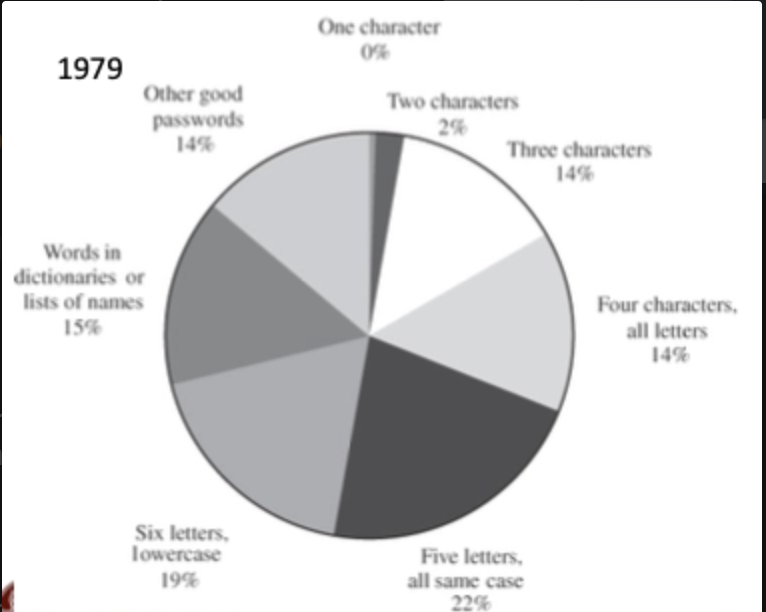
\includegraphics[width=\textwidth]{Screenshot 2026-05-03 alle 17.13.27.png}
\end{minipage}

\vspace{0.8cm}

\section*{Le strategie degli attaccanti}

\begin{quote}
    Gli attaccanti sfruttano le caratteristiche psicologiche degli utenti a proprio vantaggio poiché gli utenti solitamente evitano password lunghe, non comuni o difficili da compitare/pronunciare. Inoltre l'attaccante cercherà di ridurre lo "spazio di ricerca". Se le persone preferiscono password brevi, l'attaccante le proverà in ordine di lunghezza.
\end{quote}

Gli attaccanti sfruttano queste debolezze tramite:

\begin{itemize}
    \item \textbf{Dictionary Attack:} utilizzo di liste specializzate che includono nomi di fantascienza, luoghi, termini mitologici e parole in varie lingue.
    \item \textbf{Inferenza:} gli utenti preferiscono password brevi, facili da scrivere e da pronunciare. Un attaccante riduce lo spazio di ricerca provando le password in ordine di lunghezza. Per Esempio:
    
    \begin{equation*}
        \text{esistono solo } 26^1 + 26^2 + 26^3 \text{ combinazioni alfabetiche di lunghezza } \ge 3
    \end{equation*}

    \vspace{0.3cm}
    \item \textbf{Rainbow Tables:} I sistemi operativi non salvano le password in chiaro, ma in forma "oscurata" (tramite cifratura o hashing). Se un attaccante ottiene la tabella delle password oscurate, può violarla senza interagire con il sistema:
\end{itemize}

\vspace{0.2cm}
\noindent \begin{minipage}{0.48\textwidth}
    \begin{itemize}
        \item Costruisce una \textbf{RAINBOW TABLE}: una tabella pre-calcolata che contiene coppie di "password in chiaro" (tratte da dizionari) e i relativi "valori oscurati".
        \item Confronta i valori oscurati rubati con quelli nella Rainbow Table.
        \item Quando trova una corrispondenza, ottiene istantaneamente la password in chiaro.
    \end{itemize}
\end{minipage}
\hfill
\begin{minipage}{0.48\textwidth}
    \centering
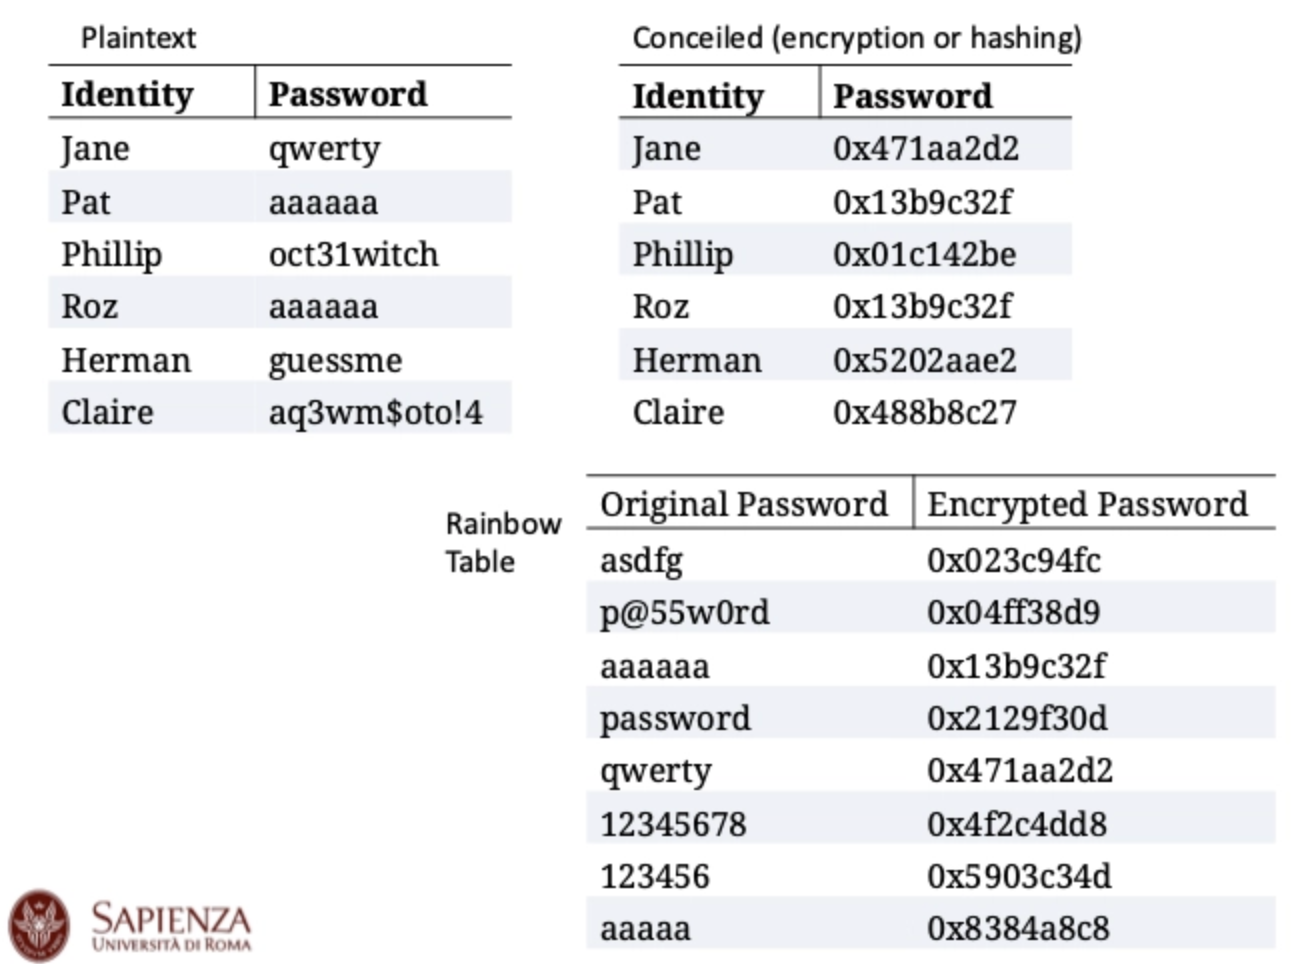
\includegraphics[width=\textwidth]{Screenshot 2026-05-03 alle 17.13.49.png}
\end{minipage}

\vspace{0.5cm}
\begin{itemize}
    \item \textbf{Brute Force:} l'attaccante prova tutte le combinazioni di password possibili.
\end{itemize}

\vspace{0.8cm}

\section*{La contromisura per il Rainbow: SALT}

Il problema principale dell'oscuramento semplice è che password uguali generano valori oscurati identici. Per contrastare le Rainbow Table, si introduce il \textbf{Salt}:

\vspace{0.3cm}
\noindent \begin{minipage}{0.48\textwidth}
    \begin{itemize}
        \item È un campo dati extra unico per ogni utente (es. data di creazione account, parte del nome o valore casuale).
        \item Viene unito alla password prima del processo di hash.
    \end{itemize}

    \vspace{0.3cm}
    \textbf{I vantaggi sono molteplici:} impedisce che password uguali siano visibili come tali, rende impossibile sapere se un utente usa la stessa password su più sistemi e aumenta la difficoltà degli attacchi offline di un fattore $2^b$, dove b è il numero di bit del salt.
\end{minipage}
\hfill
\begin{minipage}{0.48\textwidth}
    \centering
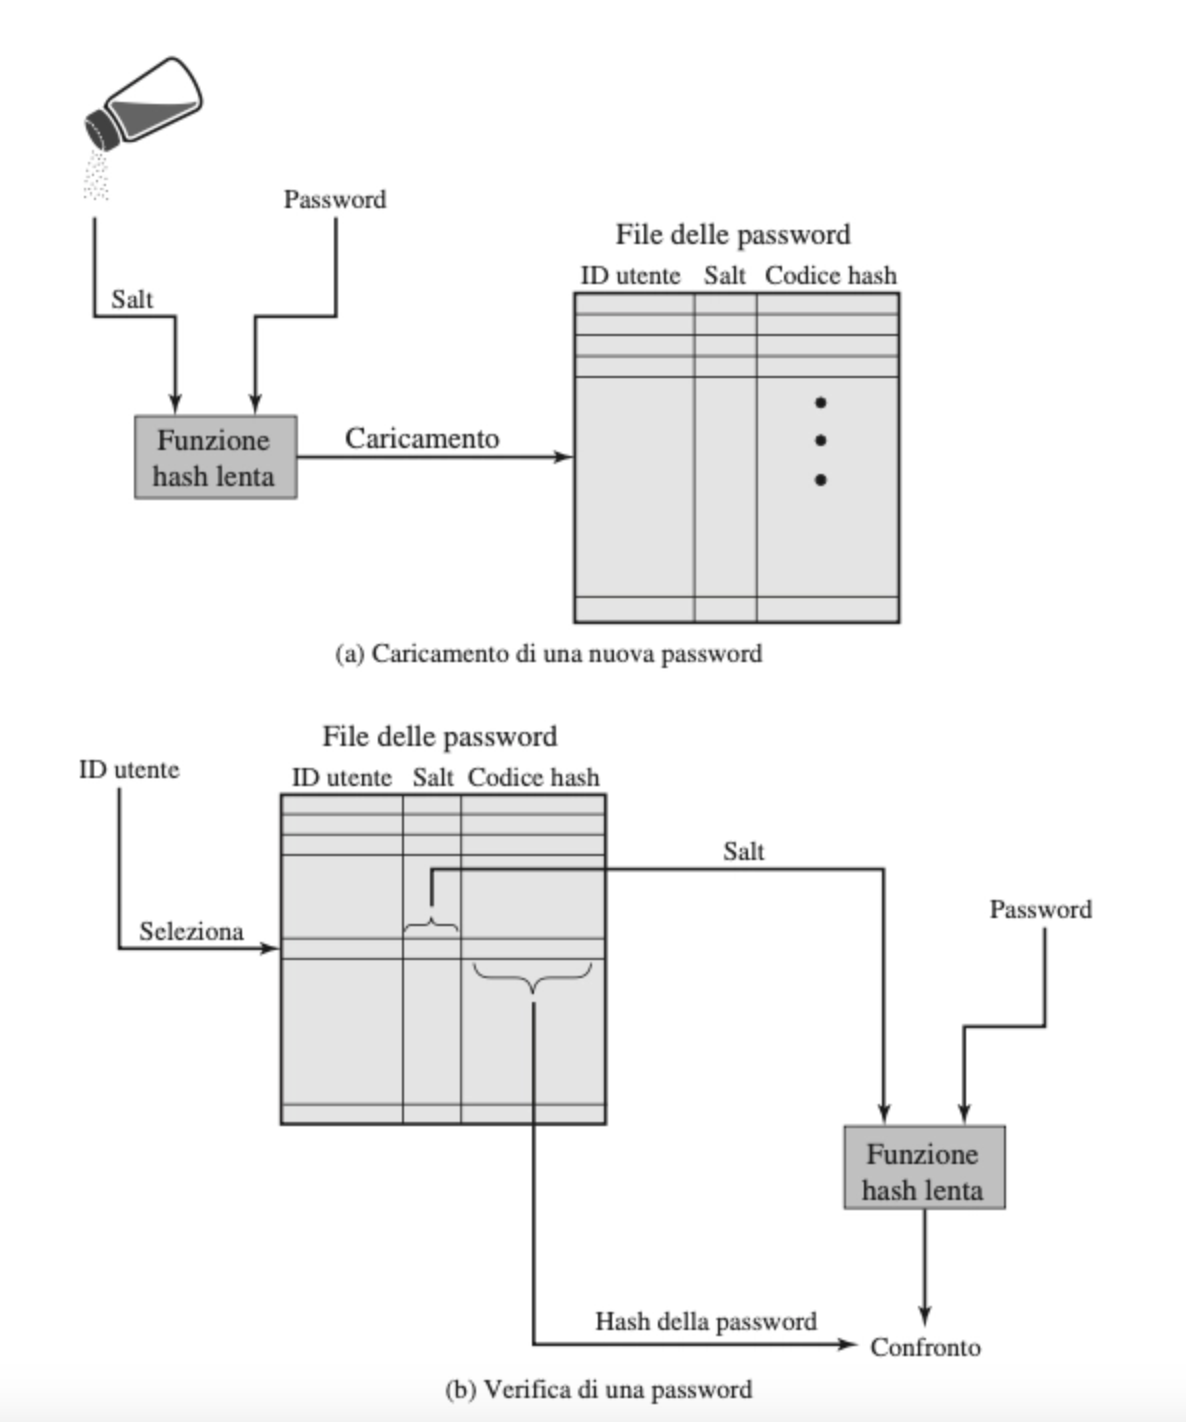
\includegraphics[width=\textwidth]{Screenshot 2026-05-03 alle 17.14.02.png}
\end{minipage}

\vspace{0.8cm}

\section*{Autenticazione Biometrica}

La biometria utilizza caratteristiche fisiche o comportamentali: impronte digitali, geometria della mano, retina, iride, voce, firma, dinamica di digitazione o vasi sanguigni.

\begin{itemize}
    \item \textbf{Vantaggi:} non può essere persa, rubata o dimenticata; è sempre disponibile ed è difficile (ma non impossibile) da falsificare.
    \item \textbf{Funzionamento:} richiede la registrazione di un "template" (modello) delle caratteristiche del soggetto. Durante l'autenticazione, le nuove misurazioni vengono confrontate con il template.
\end{itemize}

\subsection*{Test Dicotomici e Prestazioni}

L'autenticazione ha successo se il match è "abbastanza vicino" (es. 90\% di corrispondenza o parametri entro il 5\% di tolleranza). Questo è un \textbf{test dicotomico}: o c'è un match, o non c'è. I risultati possibili sono:

\begin{itemize}
    \item \textbf{True Positive (tp):} Corretto riconoscimento dell'utente legittimo.
    \item \textbf{False Positive (fp):} Errore critico per la sicurezza; un impostore viene accettato.
    \item \textbf{False Negative (fn):} Errore critico per l'usabilità; l'utente legittimo viene rifiutato.
    \item \textbf{True Negative (tn):} Corretto rifiuto di un impostore.
\end{itemize}

\vspace{0.3cm}
\noindent Le metriche di valutazione includono:

\vspace{0.3cm}
\noindent \begin{minipage}{0.48\textwidth}
    \textbf{Sensibilità:} Misura la proporzione di risultati positivi tra tutti i possibili match corretti (la capacità di identificare correttamente il soggetto cercato).
\end{minipage}
\hfill
\begin{minipage}{0.48\textwidth}
    \begin{equation*}
        \frac{tp}{tp + fn}
    \end{equation*}
\end{minipage}

\vspace{0.3cm}
\noindent \begin{minipage}{0.48\textwidth}
    \textbf{Specificità:} Misura la proporzione di risultati negativi tra tutte le persone che non sono il soggetto cercato (la capacità di escludere correttamente gli impostori).
\end{minipage}
\hfill
\begin{minipage}{0.48\textwidth}
    \begin{equation*}
        \frac{tn}{fp + tn}
    \end{equation*}
\end{minipage}

\vspace{0.3cm}
\noindent \begin{minipage}{0.48\textwidth}
    \textbf{Accuratezza:} Misura il grado in cui il test segnala correttamente la condizione o situazione complessiva.
\end{minipage}
\hfill
\begin{minipage}{0.48\textwidth}
    \begin{equation*}
        \frac{tp + tn}{tp + tn + fp + fn}
    \end{equation*}
\end{minipage}

\vspace{0.3cm}
\noindent \begin{minipage}{0.48\textwidth}
    \textbf{Prevalenza:} Indica quanto è comune una determinata condizione o situazione all'interno della popolazione del test.
\end{minipage}
\hfill
\begin{minipage}{0.48\textwidth}
    \begin{equation*}
        \frac{tp + fn}{tp + tn + fp + fn}
    \end{equation*}
\end{minipage}

\vspace{0.5cm}
Sensibilità e specificità sono legate statisticamente: se una aumenta, l'altra diminuisce. Ridurre i falsi positivi aumenterà inevitabilmente i falsi negativi. Il compromesso è rappresentato dalla curva \textbf{ROC (Receiver Operating Characteristic)}.

\subsection*{Limiti della Biometria}

La biometria può essere intrusiva e rappresenta un "single point of failure". L'accuratezza è limitata dalla velocità di riconoscimento necessaria e dalla possibilità di falsificazioni. Inoltre, è un meccanismo \textbf{debole per l'identificazione} (cercare un match tra tutti i template) a meno che ogni template non sia unico, ma \textbf{forte per l'autenticazione} (confronto con un template specifico).

\vspace{0.8cm}

\section*{Token e Identità Federata}

I token si dividono in:

\begin{itemize}
    \item \textbf{Passivi:} il contenuto non cambia (es. chiavi fisiche, foto).
    \item \textbf{Attivi:} possono variare o interagire con l'ambiente (es. smart card, RFID).
    \item \textbf{Dinamici:} generano valori imprevedibili (pass-number) che cambiano nel tempo o su richiesta, eliminando la vulnerabilità allo \textbf{skimming} (copia furtiva dei dati tramite dispositivi appositi).
\end{itemize}

\subsection*{FIM e SSO}

\begin{itemize}
    \item \textbf{Federated Identity Management (FIM):} unione di sistemi di identificazione separati che condividono un unico profilo e database di identità autenticate.
    \item \textbf{Single Sign-On (SSO):} procedura "ombrello" che gestisce identità e codici per diversi processi, permettendo all'utente di loggarsi una sola volta per sessione.
    \item \textbf{Multi-factor Authentication (MFA):} combinazione di più approcci (es. password + token dinamico). Sebbene più sicura, aumenta la complessità e può frustrare l'utente se il numero di fattori n è troppo elevato.
\end{itemize}

\vspace{0.8cm}

\section*{Riepilogo dei Rischi di Sicurezza}

\begin{table}[h!]
    \centering
    \renewcommand{\arraystretch}{1.5}
    \begin{tabularx}{\textwidth}{|l|X|}
        \hline
        \textbf{Attacco} & \textbf{Bersaglio e Caratteristiche} \\ \hline
        \textbf{Denial of Service} & Inonda il servizio di autenticazione per disabilitarlo. Può mirare a bloccare utenti specifici tramite i meccanismi di lockout. \\ \hline
        \textbf{Eavesdropping} & Tentativo di apprendere la password tramite vicinanza fisica (shoulder surfing) o keylogging. \\ \hline
        \textbf{Host Attack} & Diretto al file dei server dove sono memorizzati password, codici token o template biometrici. \\ \hline
        \textbf{Trojan Horse} & Un'applicazione o un dispositivo fisico che si maschera da autentico per catturare le credenziali. \\ \hline
        \textbf{Client Attack} & L'attaccante cerca di autenticarsi senza accedere al server o al canale di comunicazione, mascherandosi da utente legittimo. \\ \hline
        \textbf{Replay Attack} & Ripetizione di una risposta di autenticazione precedentemente catturata. \\ \hline
    \end{tabularx}
\end{table}

\end{document}